\documentclass[tikz,border=3mm]{standalone}
\usepackage{tikz}
\usetikzlibrary{angles,quotes,calc,intersections}
\begin{document}
% TikZ 1
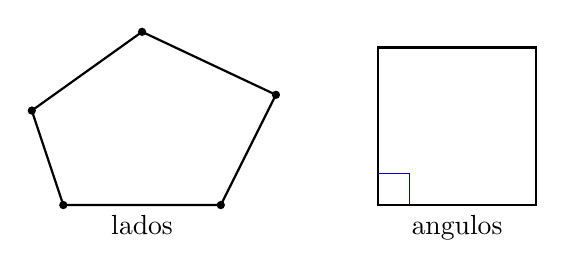
\begin{tikzpicture}[scale=1]
\draw[thick] (0,0)--(2,0)--(2.7,1.4)--(1,2.2)--(-.4,1.2)--cycle;
\node[below] at (1,0) {lados};
\foreach \p in {(0,0),(2,0),(2.7,1.4),(1,2.2),(-.4,1.2)}{\fill \p circle (1.5pt);}
\coordinate (A) at (4,0); \coordinate (B) at (6,0); \coordinate (C) at (6,2); \coordinate (D) at (4,2);
\draw[thick] (A)--(B)--(C)--(D)--cycle;
\pic[draw=blue!70!black, angle radius=4mm] {right angle=D--A--B};
\node[below] at (5,0) {angulos};
\end{tikzpicture}
\hspace{1cm}
% TikZ 2
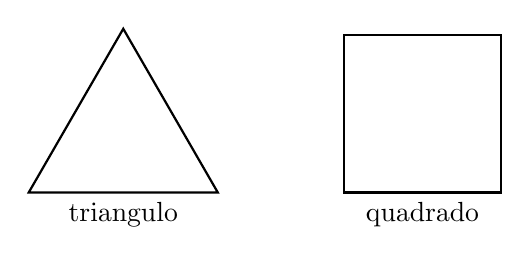
\begin{tikzpicture}[scale=1]
\coordinate (A) at (0,0); \coordinate (B) at (2.4,0); \coordinate (C) at (1.2,2.078);
\draw[thick] (A)--(B)--(C)--cycle;
\node[below] at (1.2,0) {triangulo};
\draw[thick] (4,0) rectangle (6,2);
\node[below] at (5,0) {quadrado};
\end{tikzpicture}

\vspace{1cm}

% TikZ 3
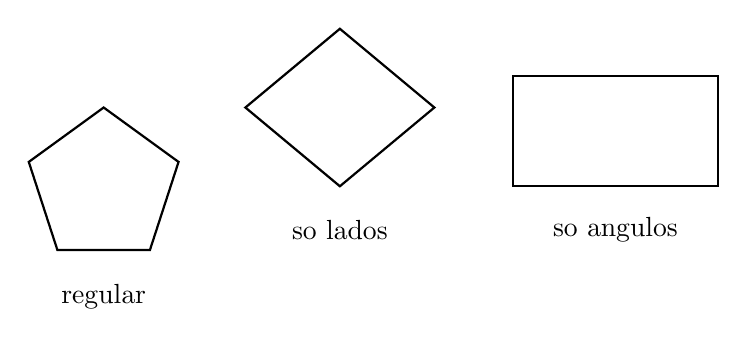
\begin{tikzpicture}[scale=1]
\foreach \k in {1,...,5}{\coordinate (P\k) at ({90+72*(\k-1)}:1);}
\draw[thick] (P1) -- (P2) -- (P3) -- (P4) -- (P5) -- cycle;
\node at (0,-1.4) {regular};
\draw[thick] (3,0)--(4.2,1)--(3,2)--(1.8,1)--cycle;
\node at (3,-.55) {so lados};
\draw[thick] (5.2,0) rectangle (7.8,1.4);
\node at (6.5,-.55) {so angulos};
\end{tikzpicture}
\hspace{1cm}
% TikZ 4
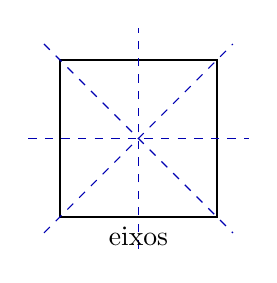
\begin{tikzpicture}[scale=1]
\draw[thick] (0,0) rectangle (2,2);
\draw[blue!70!black,dashed] (1,-.4)--(1,2.4);
\draw[blue!70!black,dashed] (-.4,1)--(2.4,1);
\draw[blue!70!black,dashed] (-.2,-.2)--(2.2,2.2);
\draw[blue!70!black,dashed] (-.2,2.2)--(2.2,-.2);
\node[below] at (1,0) {eixos};
\end{tikzpicture}

\vspace{1cm}

% TikZ 5
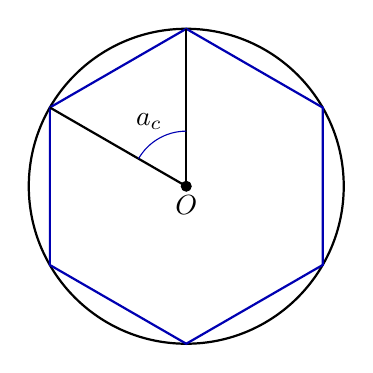
\begin{tikzpicture}[scale=1]
\coordinate (O) at (0,0);
\draw[thick] (O) circle (2);
\foreach \k in {1,...,6}{\coordinate (P\k) at ({90+60*(\k-1)}:2);}
\draw[thick,blue!70!black] (P1)--(P2)--(P3)--(P4)--(P5)--(P6)--cycle;
\draw[thick] (O)--(P1);
\draw[thick] (O)--(P2);
\pic[draw=blue!70!black, "$a_c$", angle radius=7mm, angle eccentricity=1.35] {angle=P1--O--P2};
\fill (O) circle (2pt);
\node[below] at (O) {$O$};
\end{tikzpicture}
\end{document}
